\section{Homepage}
	\subsection{Le 6W}
	\begin{figure}[H]
	\centering
	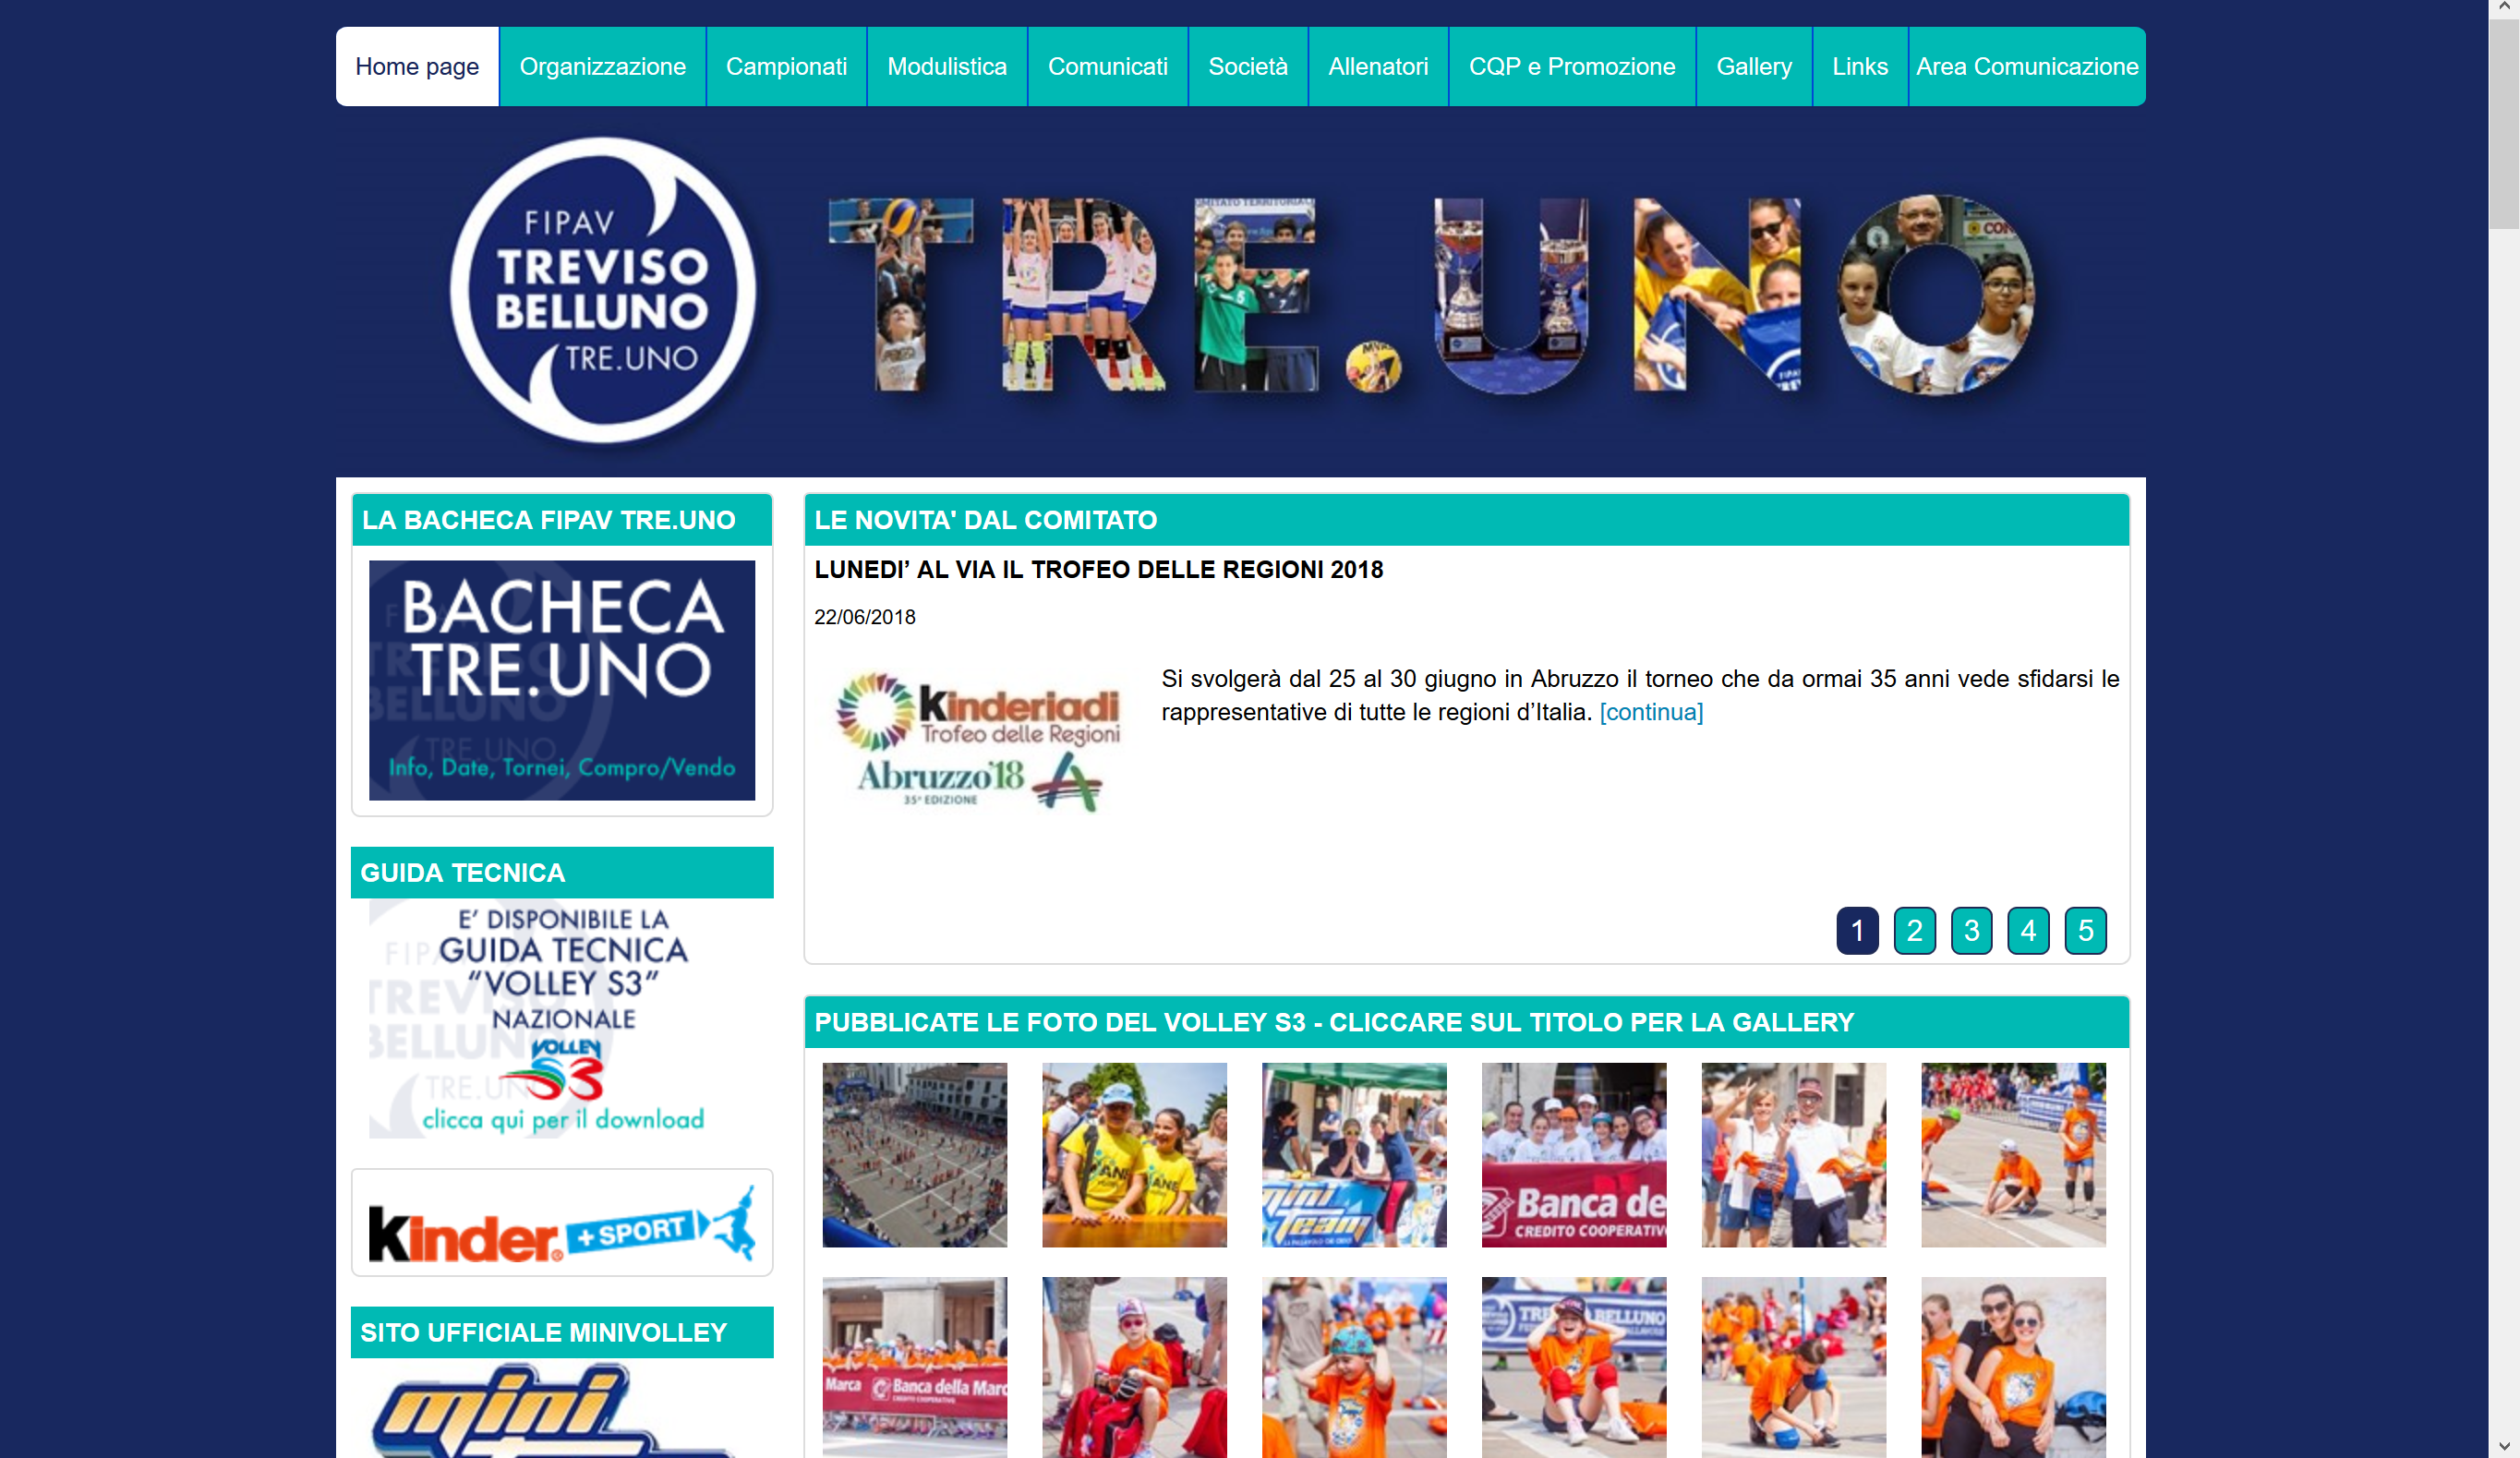
\includegraphics[scale=0.5]{Images/homepage.png}
	\caption{Homepage del sito}
	\end{figure}
	
	La homepage di un sito web dovrebbe sempre rispondere alle 6W giornalistiche, 
	un po' riadattate al contesto del web.
	
	\subsubsection{Where}
	L'asse \textit{where} indica in che tipo di sito sono arrivato. Il primo impatto
	fornisce indicazioni sul contenuto del sito web, infatti troviamo in questa 
	homepage molte notizie e foto relative a diversi campionati e tornei di
	pallavolo.
	Il logo riprende il nome del sito e le immagini da cui è composto non lasciano 
	dubbi sul tipo di sito in cui si è entrati. L'utente deve compiere diversi scroll
	per arrivare alla fine della pagina.
	Nel fondo, il sito presenta un link per collegarsi alla pagina Facebook e altri
	link utili sempre relativi alle società Fipav degli altri territori.
	
	\subsubsection{Who}
	L'asse who indica chi rappresenta il sito web. In alto a sinistra è possibile
	vedere il logo del sito web con vicino il nome. Tale logo è posizionato sotto il
	menù orizzontale e una volta che l'utente inizia a scrollare la pagina, essi non
	sono più visibili.
	La prima voce del menù è \textit{Organizzazione} in cui è presente un menù a 
	tendina con diverse sezioni in cui sono presenti i gruppi di persone coinvolte
	nell'organizzazione Fipav.
	
	\subsubsection{Why}
	L'asse why deve esporre i benefici del sito web. Come sopra citato il sito si
	occupa dell'organizzazione e l'informazione dei campionati di pallavolo 
	del territorio trevigiano e bellunese. Tale asse è soddisfatto dalle sezioni 
	presenti all'interno della hopegame, quali \textit{Novità del compitato}, 
	\textit{Nuovi contatti telefonici del comitato}, \textit{Tutte le finali dei 
	campionati ufficiali}. Inoltre, si può dire che, l'asse sia soddisfatto anche
	dalla presenza delle voci nel menù \textit{Campionati}, \textit{Modulistica} e 
	\textit{Comunicati}. 
	
	\subsubsection{What}
	L'asse what indica cosa il sito offre. Le offerte del sito web sono abbastanza
	evidenti: infatti subito si vedono le immagini relative a notizie degli 
	eventi principali. Infatti, scendendo nella pagina, si possono trovare
	gli avvisi relative alle ultime partite relative ai diversi campionati.
	Anche in questo caso l'identificazione di tale asse è semplificata dal
	menù.
	
	\subsubsection{When}
	L'asse when indica le novità temporali relative al sito. Questo è l'asse
	sicuramente più evidente dato che è un sito che propone notizie relative ai 
	campionati in corso. È possibile notare, inoltre, come queste siano ordinate
	cronologicamente dall'alto verso il basso nella pagina. In più la prima sezione
	presente nella pagina è proprio quella relativa alle novità che scorre 
	automaticamente gli ultimi eventi inseriti.
	
	\subsubsection{How}
	L'asse how ha il compito di indicare come arrivare alle sezioni principali del
	sito. Questo asse è visibile fin dall'inizio nel menù orizzontale posto sopra
	il logo. Purtroppo non è presente nessuna barra di ricerca che sarebbe stata 
	utile per ridurre il tempo dell'utente per giungere all'informazione desiderata.
	
	\subsection{Considerazioni generali}
	Il logo della pagina che forma la scritta \textbf{TRE.UNO} è stato fatto 
	unendo una serie di foto diverse, dove si mescolano diversi colori senza 
	creare un forte contrasto con lo sfondo e generando un certo sovraccarico 
	cognitivo per l'utente.
	La homepage del sito web è organizzata con una visualizzazione a griglia delle
	notizie in ordine cronologico. Tale organizzazione, anche se più compatta, è
	svantaggiosa per l'utente poiché comporta una maggiore fatica nella ricerca di
	una	particolare notizia e una seguente perdita di tempo.
	Inoltre le ultime notizie della homepage appaiono solo dopo 4/5 scroll. Tale 
	scelta è negativa in quanto:
	\begin{itemize}
		\item[•]un utente medio è disposto a scrollare per 1,3 schermi, per un totale
		 quindi di 2,3 schermi: in questo modo possono essere perse molte delle
		 notizie, anche recenti;
		\item[•]non rispetta i timer degli utenti: gli utenti in media passano 31
		  secondi nella prima pagina la prima volta che visitano il sito, che
		  diminuisce nelle visite successive stabilizzandosi intorno ai 19 secondi.
		  Ciò fa si che l'asse when non possa essere soddisfatto a pieno,
  		  considerando che un utente difficilmente accede a tutte le ultime notizie;
	\end{itemize}	
	In generale potrebbe essere preferibile spezzare tale scroll in più pagine.
	Per concludere, la homepage potrebbe essere snellita evitando di riportare molte
	notizie che sono già presenti nelle relative sezioni, come, per esempio, la lista
	dei campionati che è presente nella pagina \textit{Campionati}.
	
	\begin{figure}[H]
	\centering
	\includegraphics[scale=0.3]{Images/fullHomepage.png}
	\caption{Homepage completa del sito}
	\end{figure}
	
	
	
	
	
	
	
	
	
	
	
	
	
	
	
	
	
